\documentclass{scu-thesis}
% \usepackage{graphicx} % for including graphics
% \usepackage{amsmath}  % for advanced typesetting of mathematics
% \usepackage{txfonts}  % for using the Times-Roman font
% \usepackage{natbib}   % for better citation styles
\usepackage{tikz}
\usetikzlibrary{arrows,positioning}
\usepackage{tikz-uml}
\usepackage{pgfgantt}
\usepackage{cleveref}
\usepackage{tabulary}
\usepackage{verbatim}
\bibliographystyle{plain}

\usepackage{array}
\newcolumntype{L}[1]{>{\raggedright\let\newline\\\arraybackslash\hspace{0pt}}p{#1}}
\newcolumntype{C}[1]{>{\centering\let\newline\\\arraybackslash\hspace{0pt}}p{#1}}
\newcolumntype{R}[1]{>{\raggedleft\let\newline\\\arraybackslash\hspace{0pt}}p{#1}}

\newif\ifethics
\ethicsfalse

% These must be set first ... the rest of the thesis commands rely on them.

\author{Alex DeBoni}
\author{Jesse Harder}
\title{GPU-Accelerated Lip-Tracking Library}
\department{Department of Computer Engineering}
\degree{Bachelor of Science in Computer Science and Engineering}


% Only bachelor's theses should have multiple authors and/or be from
% multiple departments.  Signatures required:
%
% Bachelor's theses: advisor(s), department chair(s)
% Master's theses: advisor, reader, department chair
% Doctoral theses: doctoral committee (including advisor), department chair


\begin{document}
\frontmatter
\signature{Thesis Advisor}
\signature{Thesis Reader}
\signature{Department Chair}

\maketitle
\begin{abstract}
A major part of having correct pronunciation when learning a new language is moving your lips in the correct way.
One solution to this is software which will track a student's lip movements and provide feedback.
This paper describes how we are creating a C++ library to accurately track lips in provided images.
Further, this library will attempt to use a CUDA-enabled GPU implementation to improve the algorithm's performance. It will fall back on a CPU implementation if such a GPU is not found. As a result, the lip tracking library will run on Windows, Linux, and OS X, as well as Android devices.
\end{abstract}

\tableofcontents
\listoffigures

\mainmatter
\chapter{Introduction}

\section{Background}

A major part of learning a new language is to be able to pronounce words correctly. To be able to pronounce words correctly, a student's mouth needs to make proper movements. This is difficult to teach in a classroom setting, especially when a student needs to repeat the same phrase many times. The student can become frustrated with the teacher and not want to continue, especially if he or she feels as though he or she is being viewed as incompetent by his or her peers. However, when using a computer, the student can feel more comfortable trying the same phrase over and over without embarrassment.

Currently, there are desktop and mobile applications to help with a student's pronunciation by listening to him or her speak and providing feedback. If the student does not make the correct mouth shape, however, he or she is far less likely to pronounce the word correctly. Applications that only analyze audio can, at best, only guess what the student might be doing incorrectly with his or her mouth so these applications may not provide the help the student really needs.

\section{Solution}

Our solution to this problem is a mobile application to help a student pronounce words correctly by not only listening to him or her speak and analyzing the audio, but also by watching his or her mouth and providing feedback for both the audio and video information. We have created an algorithm to accurately track lip movement. A generic tracking algorithm will not work for lip motion tracking since mouths change shape too dramatically when they move. For this reason the lip tracking algorithm that we have implemented is be specialized to mouth contours. The data provided from this software is then combined with audio input to analyze how the student may improve his or her pronunciation. For example, the application can tell the student if he or she held his or her mouth open too long or didn't open his or her mouth enough for a particular word. In the end, this tool would make it easier and faster for students learning a new language to master correct pronunciation.
\chapter{Requirements}

We had several requirements that need to be met in order to implement our desired system. These requirements can be divided into two categories. Functional requirements are those which our system must do. Generally, they can be evaluated only as either true or false, depending on whether or not the system actually does or does not do what it should. Nonfunctional requirements are those which describe the manner in which the functional requirements should be achieved. They are evaluated based on a degree of satisfaction. Additionally, our system also has a couple design constraints, which are limits on the design and implementation of the system. The following requirements were to be met for successful implementation of our lip-tracking library.

\section{Functional}
The system will:
\begin{itemize}
\item Receive camera images from the user.
\item Return a point array of lip edges.
\end{itemize}


\section{Nonfunctional}
The system will be:
\begin{itemize}
\item Efficient - it will run quickly enough for use in a real time system.
\item User Friendly - it will have an easy to use interface.
\item Reliable/accurate - it will produce correct data.
\item Robust - it won't crash. (i.e. Its crash frequency will be within acceptable norms.)
\item Reusable - it will be easy to use in other systems.
\end{itemize}


\section{Design Constraints}
The system must:
\begin{itemize}
\item Be able to run on Android devices and desktop computers.
\item Use CUDA.
\end{itemize}
\chapter{Conceptual Model}

The interface to our lip-tracking library consists of six functions. The first is the \texttt{initializeTracker} function, which takes as a parameter the file containing the shape data that the tracker uses to perform its analysis. This will allow the tracking process to start. The next two functions, \texttt{getAcceptanceThreshold} and \texttt{setAcceptanceThreshold}, allow the user to get and set a threshold value used in creating a lip contour. This threshold value determines the required confidence in the lip-tracking algorithm. The lower the threshold value, the less accurate the algorithm is. If the value is too high, however, the algorithm may fail to obtain a lip contour at the desired confidence level, resulting in an error being reported. The \texttt{getLipContour} function is used to obtain a lip contour model as an array of points. This function takes as parameters the file path to the image file to be processed and a reference to the array in which the lip contour information is to be stored. It also returns a status code indicating success or failure. The array that is passed in must have already been allocated by the user. To do this, the user will use the \texttt{getNumberOfContourPoints} function, which returns the size that the array should be. Finally, the user may also call the \texttt{resetTracker} function to tell the tracking process to re-evalute the entire image instead of just the region in which it believes the lips to be.

\section{API Functions}
\begin{itemize}
\item \texttt{void initializeTracker(char *iniFile);}
\item \texttt{int getAcceptanceThreshold();}
\item \texttt{void setAcceptanceThreshold(int threshold);}
\item \texttt{int getNumberOfContourPoints();}
\item \texttt{int getLipContour(char *filePath, float contour[]);}
\item \texttt{void resetTracker();}
\end{itemize}
\chapter{Use Cases}
Based on our conceptual model, our system has a number of actions that users might perform. Any action that a user might take can be considered a use case, which is defined as the steps needed to achieve a goal on the application. Presented below are the use cases for our library, which effectively correspond to the different functions in the library. Under each use case, the actor, goal, precondition, postcondition, sequence of steps, and exceptions are listed. All the use cases of our application are shown below in \Cref{fig:use-cases}. Following the diagram are detailed descriptions of each use case.


\begin{figure}[!h]
\noindent\centering\resizebox{0.8\textwidth}{!}{
  \begin{tikzpicture}

\begin{umlsystem}[x=4]{Use Cases} 
\umlusecase{~~~~~~~~~~Initialize Tracker~~~~~~~~~~} 
\umlusecase[y=-2]{~~~Get Acceptance Threshold~~~} 
\umlusecase[y=-4]{~~~~Set Acceptance Threshold~~~~}  
\umlusecase[y=-6]{Get Number of Contour Points}
\umlusecase[y=-8]{~~~~~~~~~~Get Lip Contour~~~~~~~~~~}
\umlusecase[y=-10]{~~~~~~~~~~~~Reset Tracker~~~~~~~~~~~~} 
\end{umlsystem} 

\umlactor[y=-5, x=-2.5]{user} 

\umlassoc{user}{usecase-1} 
\umlassoc{user}{usecase-2} 
\umlassoc{user}{usecase-3} 
\umlassoc{user}{usecase-4} 
\umlassoc{user}{usecase-5} 
\umlassoc{user}{usecase-6} 

\end{tikzpicture}
}
\caption{Use case diagram}
\label{fig:use-cases}
\end{figure}

\section{Use Case 1: Get Lip Contour}

\begin{description}
  \item[Actor:] User.
  \item[Goal:] Obtain lip contour data from a face image.
  \item[Preconditions:] User has imported our library, has an image to process, and has allocated an array of the proper size.
  \item[Postconditions:] User has a lip contour for the provided image.
  \item[Sequence of Steps:] User calls one of the \texttt{getLipContour} functions on the facial image.
  \item[Exceptions:] The image provided is not of a face: the function will return an error code.
\end{description}


\section{Use Case 2: Get Number of Contour Points}

\begin{description}
	\item[Actor:] User.
	\item[Goal:] Obtain the number of contour points provided by the lip-tracking process.
	\item[Preconditions:] User has imported our library.
	\item[Postconditions:] User has the number of contour points.
	\item[Sequence of Steps:] User calls the \texttt{getNumberOfContourPoints} function.
	\item[Exceptions:] None.
\end{description}


\section{Use Case 3: Get Acceptance Threshold}

\begin{description}
  \item[Actor:] User.
  \item[Goal:] Obtain a value for the acceptance threshold for the lip tracking process.
  \item[Preconditions:] User has imported our library.
  \item[Postconditions:] User has acceptance threshold value.
  \item[Sequence of Steps:] User calls the \texttt{getAcceptanceThreshold} function.
  \item[Exceptions:] None.
\end{description}


\section{Use Case 4: Set Acceptance Threshold}

\begin{description}
  \item[Actor:] User.
  \item[Goal:] Change the value for the acceptance threshold for the lip tracking process.
  \item[Preconditions:] User has imported our library.
  \item[Postconditions:] Acceptance threshold value is changed to provided value.
  \item[Sequence of Steps:] User calls the \texttt{setAcceptanceThreshold} function.
  \item[Exceptions:] User provides an invalid value to the function: acceptance threshold value will remain unchanged. Function will return 1 to indicate failure.
\end{description}
\chapter{Technologies Used}
\label{technologies}

Below we list all of the technologies that we used in our system and the basic reasons why we chose to use each of them.

\section{C++}

We used C++ because it is a relatively efficient programming language. Additionally, it allowed us to create one library that can be cross-compiled and reused on any platform. Further, both of us have a significant amount of experience with the language.

\section{CUDA}

CUDA (Compute Unified Device Architecture) is a parallel computing platform and programming model developed by Nvidia for their GPUs. We used CUDA because Android devices are now starting to get dedicated GPU chips that are optimized for CUDA.

\section{Nvidia Tegra K1}

We used the Nvidia Tegra K1 GPU because it is the currently the most common mobile GPU being marketed, with phones like the Google Nexus 9 utilizing it.

\section{OpenCV}

We used the OpenCV library to do image processing such as noise filtering and edge detection. 
OpenCV also detects if there is a CUDA-capable GPU on the system and will use it if it finds one.
Additionally, it is compatible with Windows, Linux, OS X, Android, and iOS, so it will work for all of our implementations.

\section{CMake}

CMake is a cross-platform make utility which detects what compilers are installed on the system and selects an appropriate to use for the project. This made it easy for us to test changes on different platforms by streamlining the compilation process.
\chapter{Design Rationale}

In this chapter we list and explain the reasoning for the design choices we have made for the lip-tracking library.

\section{Technologies}

A description of the technologies we will be using can be found in \Cref{technologies}. We chose these technologies because they are very common and well supported, in addition to being available on every platform we are working with (Windows, Linux, OS X, Android). 

\section{Application Programming Interface}

We wanted to make our API as simple as possible for the user, while still being flexible. As a result, we allow images to inputted in three different formats: Portable Grey Map (PGM), Portable Pixel Map (PPM), and Bitmap (BMP). These formats allow for both color (BMP and PPM) and greyscale (PGM) images, in formats that are very common. 

The user can also change the acceptance threshold for lip detection. If there are too many false positives, then the threshold can be lowered to compensate, and vice versa.

\section{Algorithm}

There are many different algorithms that have been used in the past for feature tracking. 
These can be divided into three categories, geometric-based approaches, appearance-based approaches, and model-based approaches. Ahmad Hassanat has provided a literature review comparing these approaches in his paper \textit{Visual Speech Recognition}~\cite{Hassanat14}.

\subsection{Geometric-Based Approaches}

These approaches involve edge detection and then trying to match ratios of the edge's height, width, area and perimeter with some predefined values.

\subsection{Appearance-Based Approaches}

These approaches involve color segmentation of the image and then trying to match a segment with a predefined set of colors. 
This is the most common approach currently taken~\cite{Stillittano13}\cite{Yang09}, but does not always have good results. Increasing the contrast beforehand can somewhat improve the results.

\subsection{Model-Based Approaches}

These approaches involve creating a statistical model of a feature shape by inputting a set of hand-landmarked images into a neural network.
This model can then be used to very accurately find a similar shape in an image. 
There are three common model-based approaches, the Active Contour Model (ACM), Active Shape Model (ASM), and Active Appearance Model (AAM).
These three models are closely related in that they all use the same fundamental algorithm. However, ASM is an improvement over ACM and AAM is an improvement over ASM. These improvements bring more accuracy to the algorithm, however, they also increase complexity and runtime.

Additionally, both ASM~\cite{Li09} and AAM~\cite{Wang14} have been shown to be parallelizable with CUDA.
	

\subsection{Our Approach}

We have chosen to take a hybrid approach that combines all three previous approaches. The geometric-based and appearance-based approaches alone do not produce results that are accurate enough for us. They run very quickly, however, and can produce a better input image for a model-based approach. The model-based approach we are using is the Active Shape Model. The model is a good balance between the Active Contour Model, which is too simple and not accurate enough, and the Active Appearance Model, which is complicated and relatively slow. We will also convert all of the input images to grayscale as this will speed up many of the processing operations. An example of all the operations we will perform can be found in \Cref{fig:lena}.

\begin{figure}[p]
    \centering
    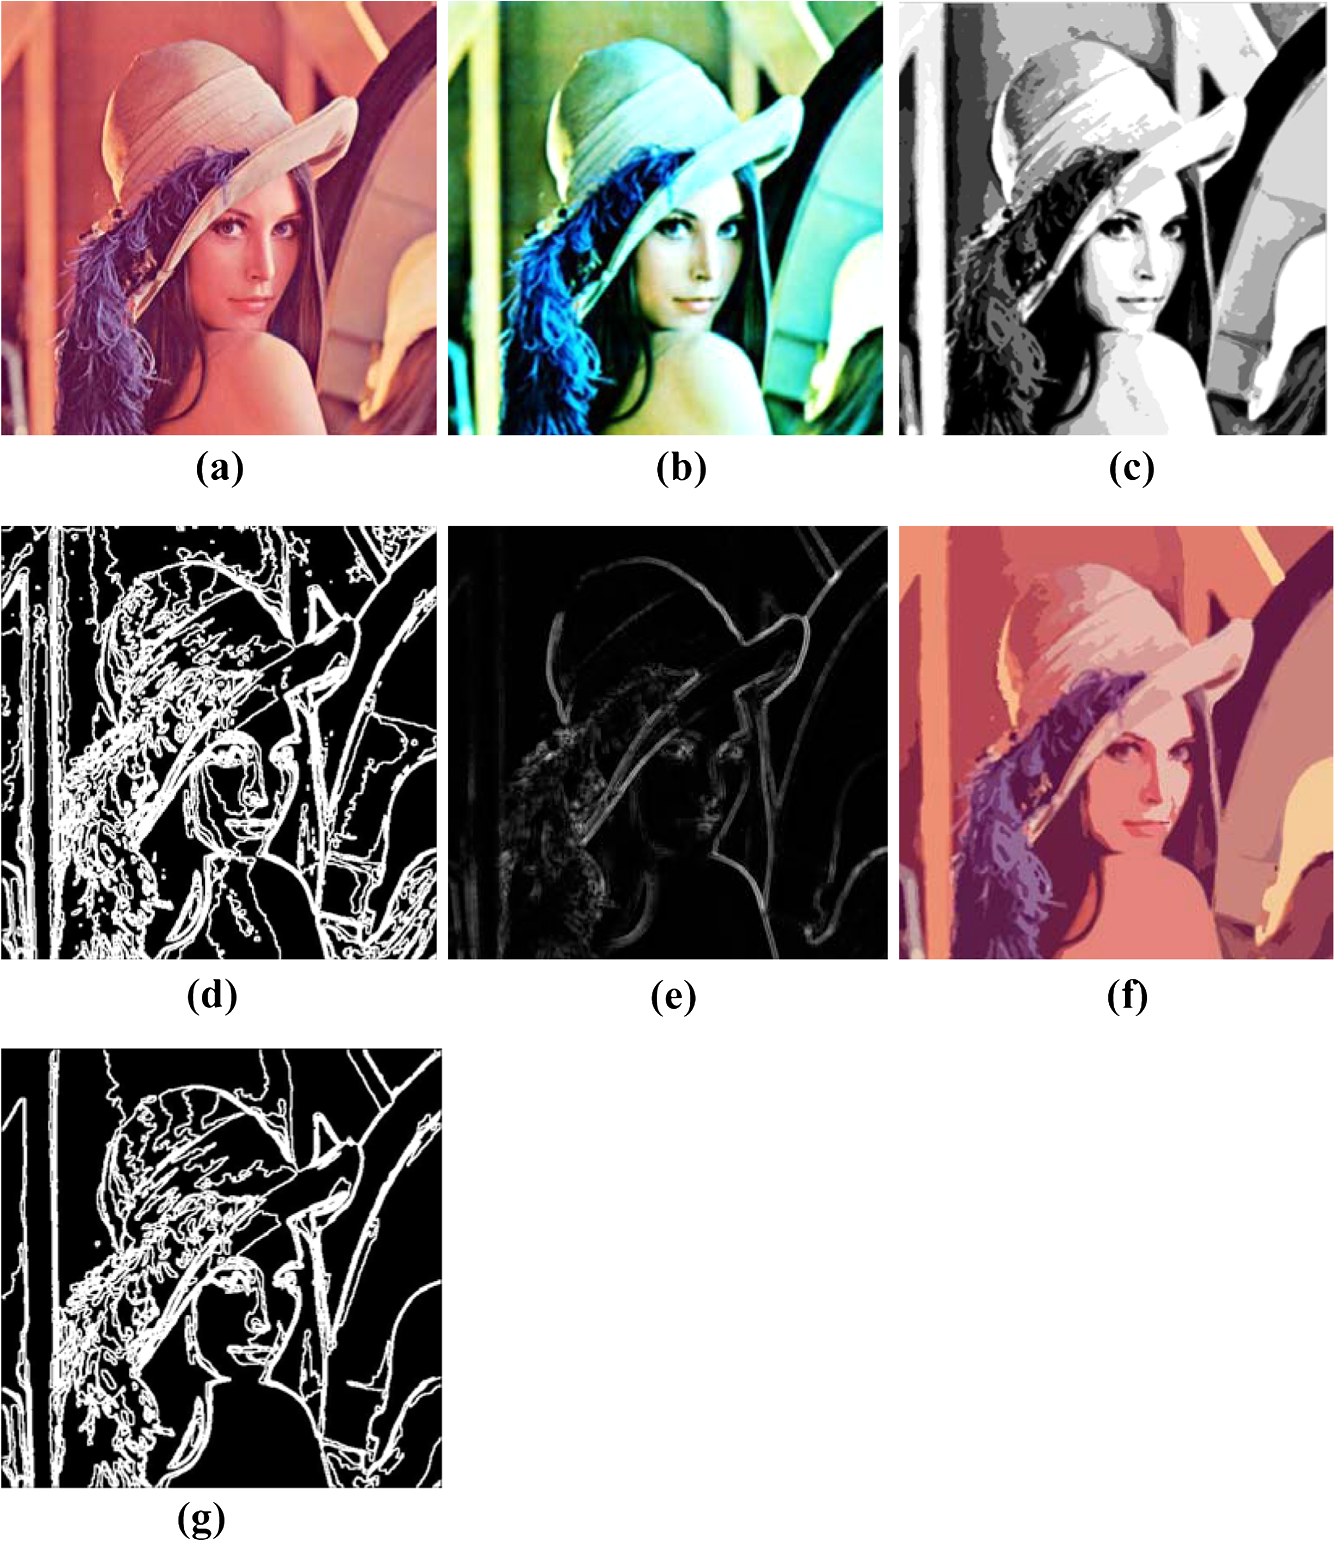
\includegraphics[width=0.8\textwidth]{diagrams/lena.png}
    \caption{(a) Source image\\(b) Increased contrast\\(c) Grayscale\\(d) Heavy edge detection\\
	(e) Light edge detection\\(f) Color segmentation\\(g) Medium edge detection\\Figure taken from Zhang\cite{filters}}
    \label{fig:lena}
\end{figure}
\chapter{Architectual Diagram}

We will be using a data-flow architecture for our system, also known as a pipe-and-filter architecture. 
The system will have an array of pixel values for an image which gets modified by each filter it passes through.
The entire data flow for our system can be seen in \Cref{fig:architecture}.
\newline

\begin{figure}[!h]
\noindent\resizebox{\textwidth}{!}{
  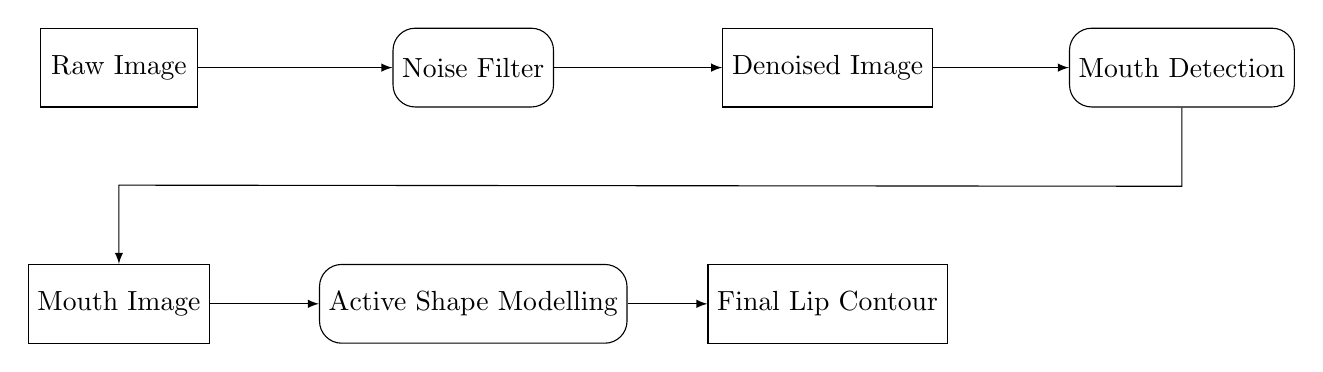
\begin{tikzpicture}[auto, node distance=1cm and 4.5cm, >=latex]
	\tikzset{
		block/.style= {draw, rectangle, align=center, minimum width=2cm, minimum height=1cm},
		rblock/.style={draw, shape=rectangle, rounded corners=0.8em, align=center, minimum width=2cm, minimum height=1cm},
	}

	\node [coordinate] (r1c1) {};
	\node [coordinate, right= of r1c1] (r1c2) {};
	\node [coordinate, right= of r1c2] (r1c3) {};
	\node [coordinate, right= of r1c3] (r1c4) {};

	\node [coordinate, below=3cm of r1c1] (r2c1) {};
	\node [coordinate, right= of r2c1] (r2c2) {};
	\node [coordinate, right= of r2c2] (r2c3) {};

	\node [block, right of=r1c1] (rawImage) {Raw Image};
	\node [rblock, right of=r1c2] (noiseFilter) {Noise Filter};
	\node [block, right of=r1c3] (quietImage) {Denoised Image};
	\node [rblock, right of=r1c4] (mouthDetection) {Mouth Detection};

	\node [block, right of=r2c1] (mouthImage) {Mouth Image};
	\node [rblock, right of=r2c2] (asmModel) {Active Shape Modelling};
	\node [block, right of=r2c3] (lipArray) {Final Lip Contour};

	\node [coordinate, below =1cm of mouthDetection] (r1end) {};
	\node [coordinate, above =1cm of mouthImage] (r2start) {}; 

	\path[draw,->] 
				(rawImage) edge (noiseFilter)
				(noiseFilter) edge (quietImage)
				(quietImage) edge (mouthDetection)

				(mouthImage) edge (asmModel)
				(asmModel) edge (lipArray)

				(mouthDetection.south) -- (r1end) -- (r2start) -- (mouthImage.north)
				;
\end{tikzpicture}
}
\caption{System architecture}
\label{fig:architecture}
\end{figure}
\chapter{Test Plan}

It was necessary for us to test our system in order to ensure that our lip-tracking library is fully functional and meets all of the requirements we have identified for it. There are a number of different ways that we planned to test our system, the main points of which are listed below.

\section{Alpha Testing}

We have a library of videos and images of people's lips. We visually analyzed the output of our program for these inputs to see how accurately it tracks the lips.

We also planned to perform automated unit testing, including the following sets of test.
\begin{itemize}
	\item Checking a variety of images that either do or do not have lips in them to see whether the library properly identifies the lips or lack thereof in the image.
	\item Iterating through a range of acceptance threshold values on various images of lips to see when detection starts and stops.
\end{itemize}

\section{Beta Testing}

We planned to get a group of people with a diverse set of facial features to test our library with a webcam and visually analyze the results.
The variables we aimed to test include mustaches, beards, teeth presence, lip color, and skin color.
\chapter{Project Risks}
\Cref{table:risks} below shows the potential risks we identified for our project. Listed with each risk are the consequences should the risk occur, the probability of the risk occurring, the severity of the risk, the impact of the risk (calculated by multiplying probability and severity), and the mitigation strategies we employed to avoid the risk from occurring.
\newline
\begin{table}[!h]
\def\arraystretch{1.5}
\begin{tabulary}{\textwidth}{|L{2.3cm}|L{2.5cm}|L{2cm}|L{1.5cm}|L{1.3cm}|L{2.9cm}|}
\hline
\textbf{Risk} & \textbf{Consequences} & \textbf{Probability} & \textbf{Severity} & \textbf{Impact} & \textbf{Mitigation} \\
\hline\hline
Poor time management & Not having a finished product. & 0.4 & 7 & 2.8 & Follow gantt chart schedule. Prioritize features of system. \\ \hline
GPU transition problems & Delays. Potentially only CPU implementation finished. & 0.3 & 8 & 2.4 & Consider GPU implementation while working on CPU version. \\ \hline
Team member becomes sick or otherwise disabled & Loss of time. & 0.4 & 4 & 1.6 & Stay informed on each other's progress.Soft deadlines. \\ \hline
Major issues with chosen technologies & Loss of time and progress. & 0.2 & 7 & 1.4 & Early testing of technologies. Consider alternative technologies in advance. \\ \hline
Failure to gather sufficient beta testers & Incomplete testing. & 0.5 & 2 & 1.0 & Scout beta testers in advance. Have thorough alpha testing plan. \\ \hline
%Explosion of the Earth's Sun & Everyone dies. & 1e-27 & 10 & 1e-26 & Pray. Say goodbye to loved one's. \\ \hline
\end{tabulary}
\caption{Risk analysis table}
\label{table:risks}
\end{table}
\chapter{Development Timeline}

The figures below show timelines of the work we have done as well as when we will be working on and finishing each major task of this project that we have yet to complete, including the writing of the library, finishing the documentation, and preparation for the final presentations in the spring. By following this plan, we have and will continue to keep ourselves on schedule for our upcoming deadline.
\newline

\begin{figure}[!h]
\noindent\resizebox{\textwidth}{!}{
  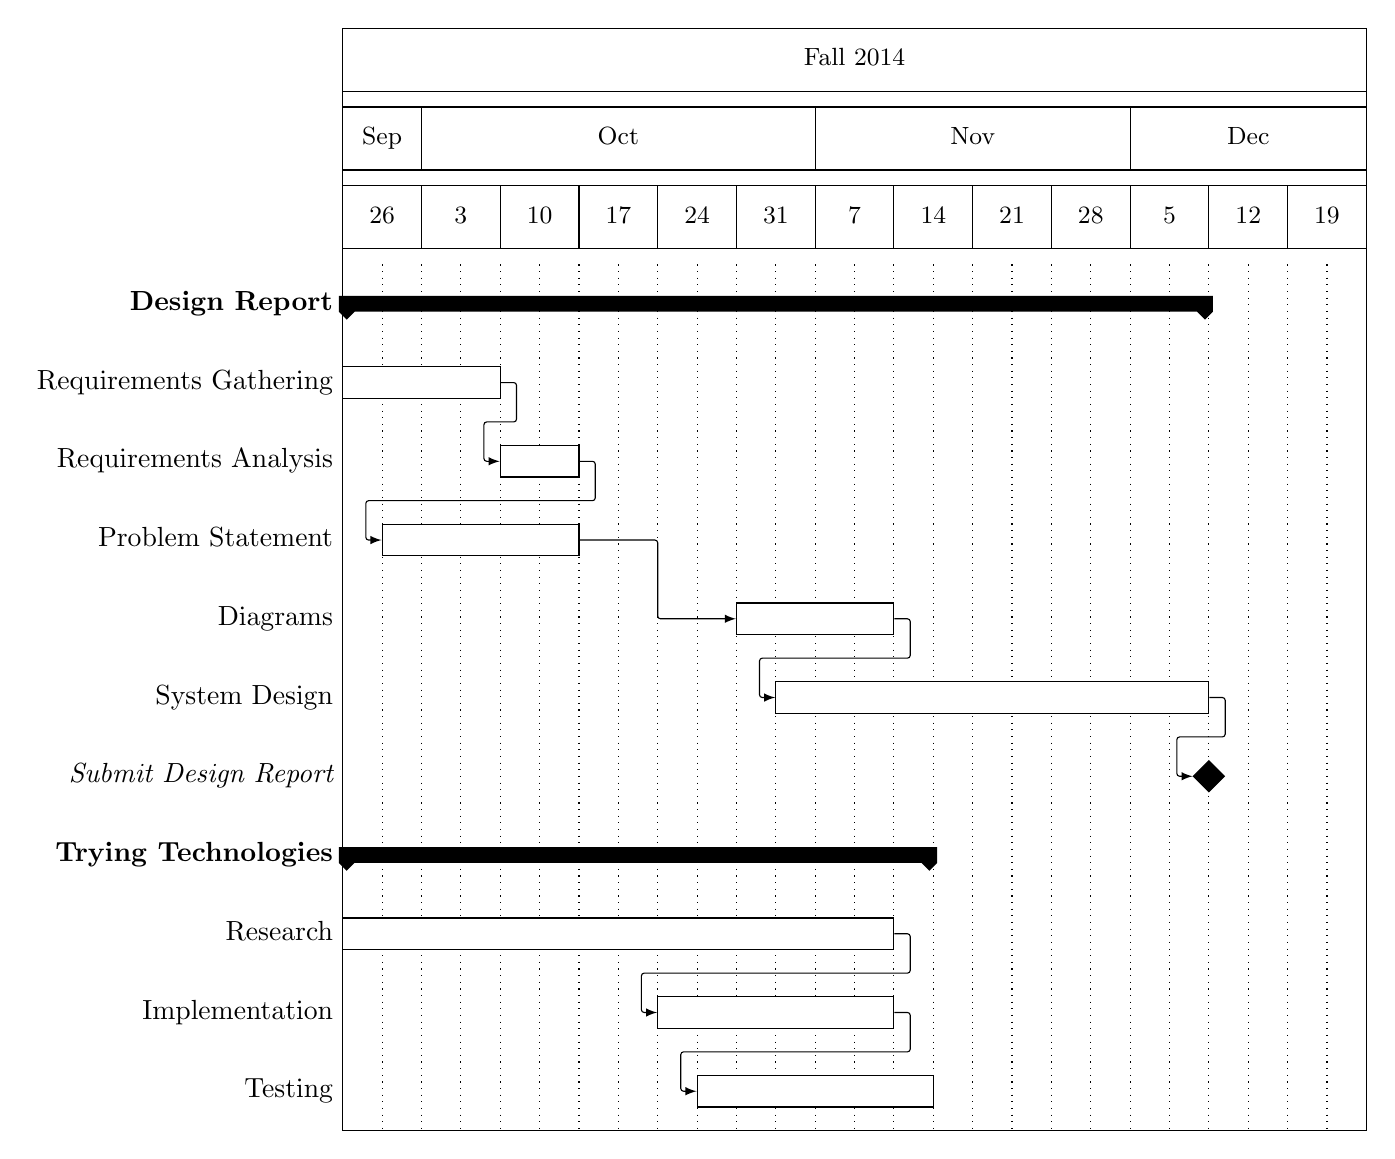
\begin{tikzpicture} 

\begin{ganttchart}[vgrid, title height=0.8]{1}{26}
  \gantttitle{Fall 2014}{26} \\
  \gantttitle{Sep}{2}
  \gantttitle{Oct}{10}
  \gantttitle{Nov}{8}
  \gantttitle{Dec}{6} \\
  \gantttitlelist{26,3,10,17,24,31,7,14,21,28,5,12,19}{2} \\

  \ganttgroup{Design Report}{1}{22} \\
  \ganttbar{Requirements Gathering}{1}{4} \\
  \ganttlinkedbar{Requirements Analysis}{5}{6} \\
  \ganttlinkedbar{Problem Statement}{2}{6} \\
  \ganttlinkedbar{Diagrams}{11}{14} \\
  \ganttlinkedbar{System Design}{12}{22} \\
  \ganttlinkedmilestone{Submit Design Report}{22} \\

  \ganttgroup{Trying Technologies}{1}{15} \\
  \ganttbar{Research}{1}{14} \\
  \ganttlinkedbar{Implementation}{9}{14} \\
  \ganttlinkedbar{Testing}{10}{15} 
\end{ganttchart}

\end{tikzpicture} 
}
\caption{Fall quarter gantt chart}
\label{fig:gantt-fall}
\end{figure}


\begin{figure}[!h]
\noindent\resizebox{\textwidth}{!}{
  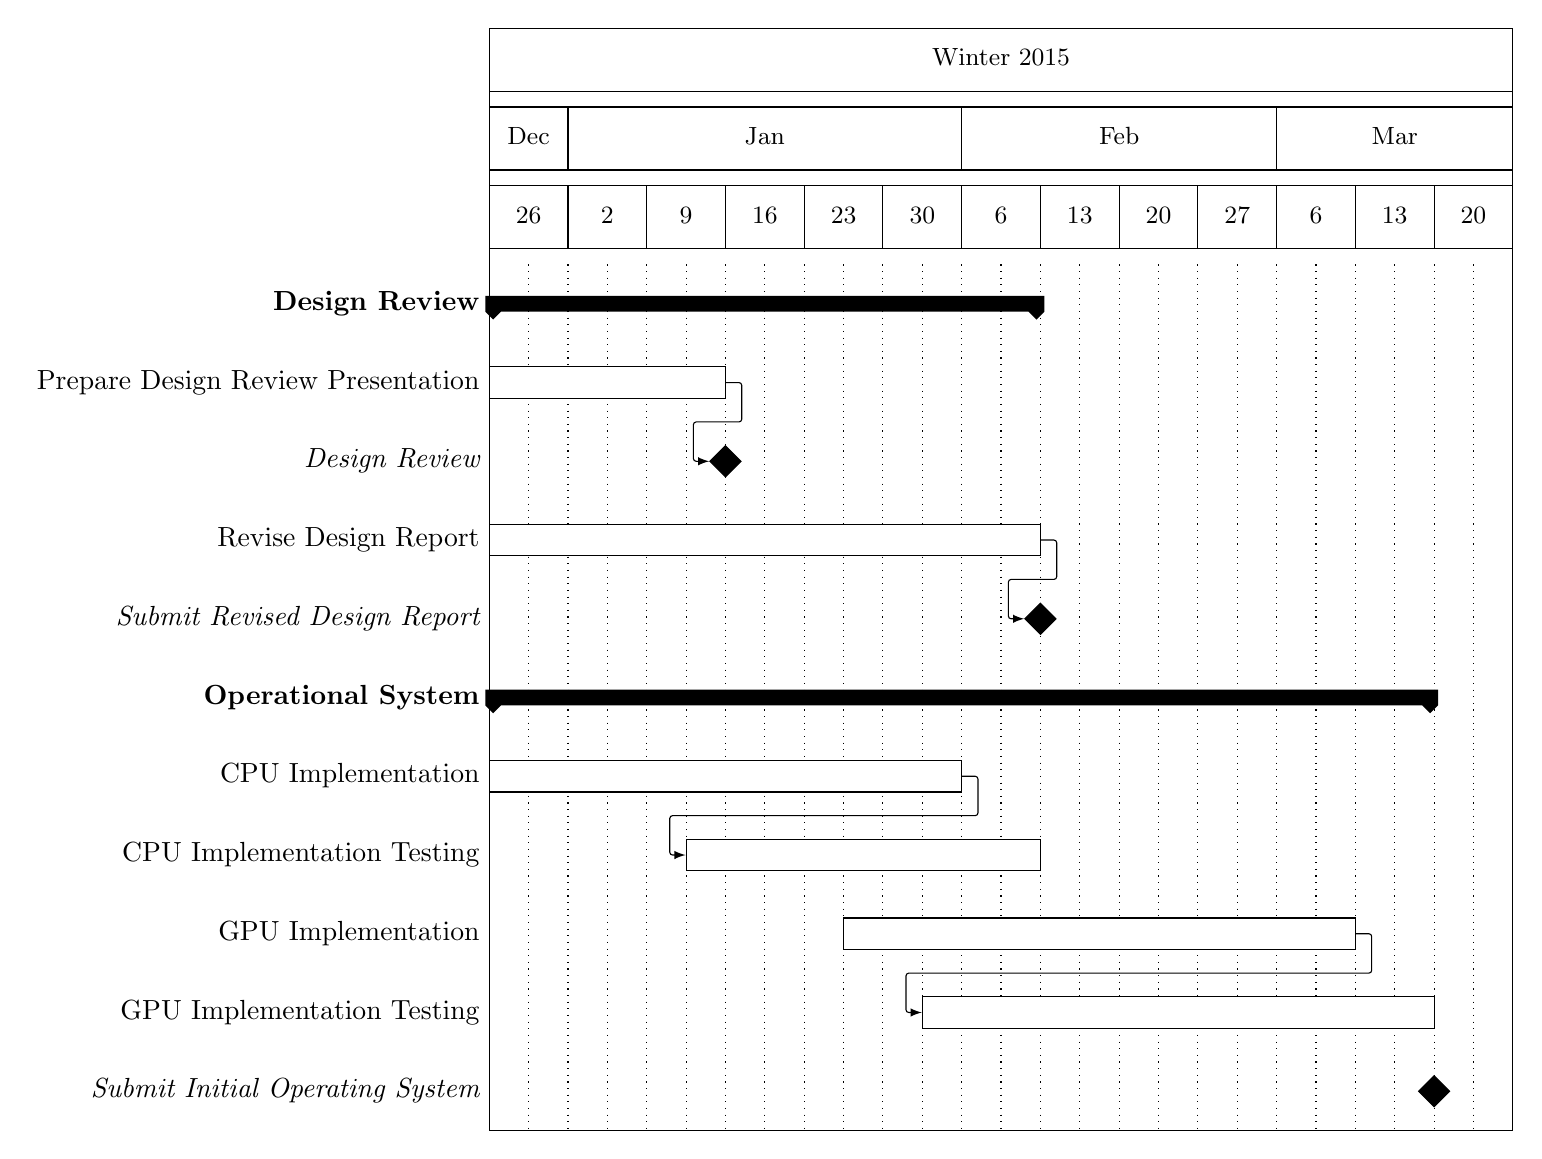
\begin{tikzpicture} 

\begin{ganttchart}[vgrid, title height=0.8]{1}{26}
  \gantttitle{Winter 2015}{26} \\
  \gantttitle{Dec}{2}
  \gantttitle{Jan}{10}
  \gantttitle{Feb}{8}
  \gantttitle{Mar}{6} \\
  \gantttitlelist{26,2,9,16,23,30,6,13,20,27,6,13,20}{2} \\

  \ganttgroup{Design Review}{1}{14} \\
  \ganttbar{Prepare Design Review Presentation}{1}{6} \\
  \ganttlinkedmilestone{Design Review}{6} \\
  \ganttbar{Revise Design Report}{1}{14} \\
  \ganttlinkedmilestone{Submit Revised Design Report}{14} \\

  \ganttgroup{Operational System}{1}{24} \\
  \ganttbar{CPU Implementation}{1}{12} \\
  \ganttlinkedbar{CPU Implementation Testing}{6}{14} \\
  \ganttbar{GPU Implementation}{10}{22} \\
  \ganttlinkedbar{GPU Implementation Testing}{12}{24} \\
  \ganttmilestone{Submit Initial Operating System}{24}
\end{ganttchart}

\end{tikzpicture}
}
\caption{Winter quarter gantt chart}
\label{fig:gantt-winter}
\end{figure}


\begin{figure}[!h]
\noindent\resizebox{\textwidth}{!}{
  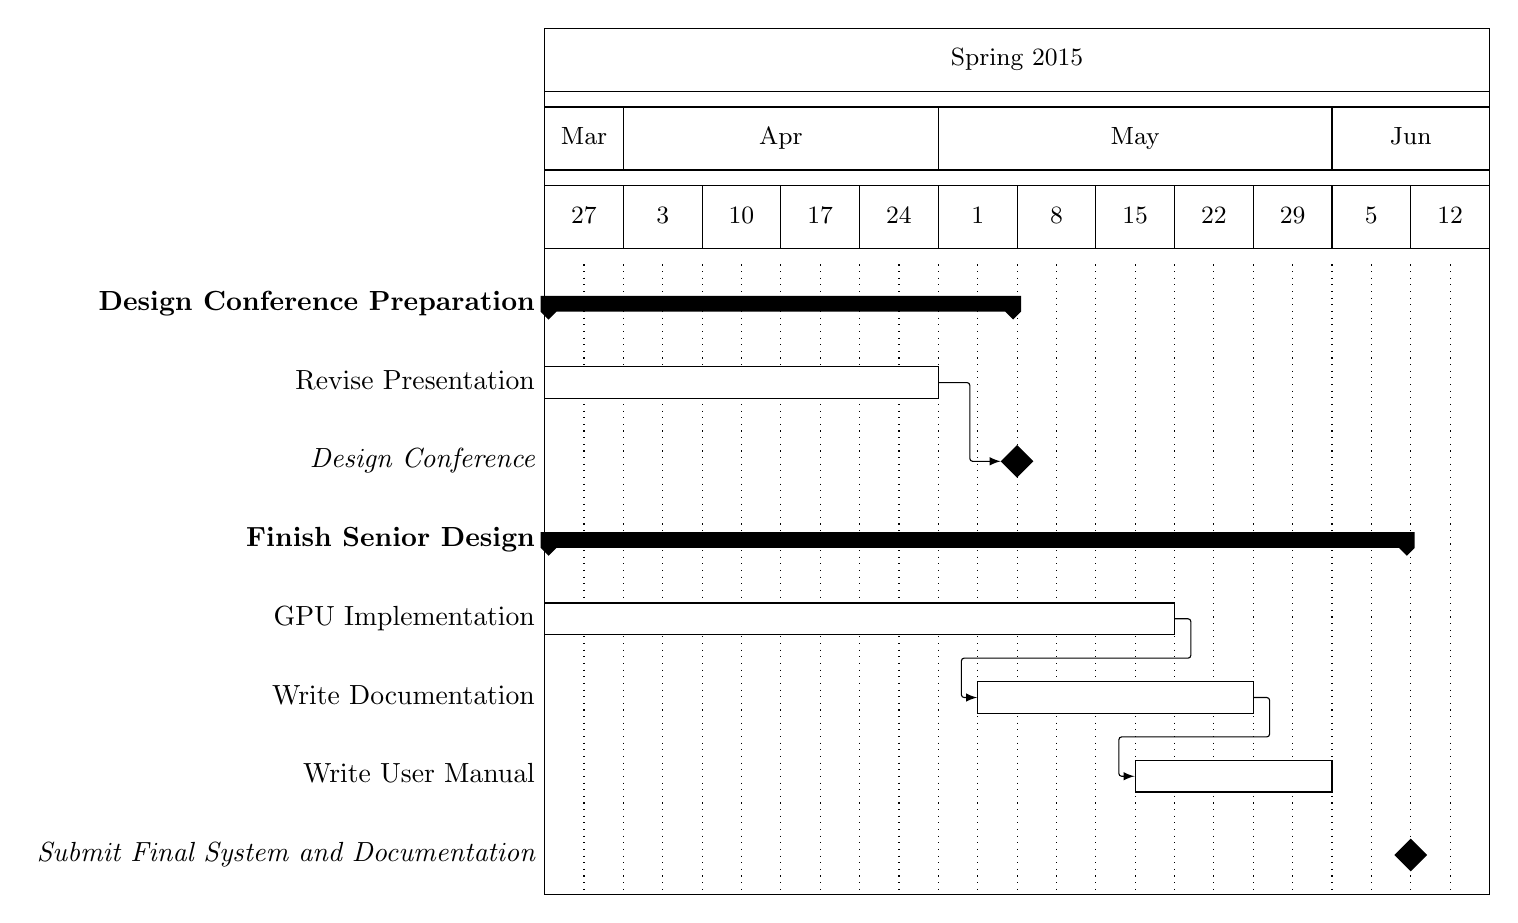
\begin{tikzpicture} 

\begin{ganttchart}[vgrid, title height=0.8]{1}{24}
  \gantttitle{Spring 2015}{24} \\
  \gantttitle{Mar}{2}
  \gantttitle{Apr}{8}
  \gantttitle{May}{10}
  \gantttitle{Jun}{4} \\
  \gantttitlelist{27,3,10,17,24,1,8,15,22,29,5,12}{2} \\

  \ganttgroup{Design Conference Preparation}{1}{12} \\
  \ganttbar{Revise Presentation}{1}{10} \\
  \ganttlinkedmilestone{Design Conference}{12} \\

  \ganttgroup{Finish Senior Design}{1}{22} \\
  \ganttbar{GPU Implementation}{1}{16} \\
  \ganttlinkedbar{Write Documentation}{12}{18} \\
  \ganttlinkedbar{Write User Manual}{16}{20} \\
  \ganttmilestone{Submit Final System and Documentation}{22}
\end{ganttchart}

\end{tikzpicture} 
}
\caption{Spring quarter gantt chart}
\label{fig:gantt-spring}
\end{figure}

\chapter{Results}

\section{Pre processing Input Images}
Our initial plan was to use a geometric based and appearance based approach to pre process the input images before doing the shape modeling step. The geometric based approach involves doing edge detection on the image, which can highlight the contours of the lips better for easier detection. The appearance based approach involves doing color segmentation on the image which can separate the lips from the rest of the face due to their different color. 

After trying these approaches, we found that they are not viable methods of enhancement. The edge detection alone did not slow down the program noticeably (it only added 10 milliseconds of processing time per frame) but it made detection much worse. The shape modeling algorithm could not find landmarks on the input image after an edge detection filter was applied to it. The color segmentation filter did not worsen the shape modeling algorithm like edge detection did, but it also did not noticeably improve shape modeling either. Also, as a downside, doing color segmentation alone takes a noticeable amount of time (40 milliseconds per frame), so it slowed down the program considerably. And finally, combining the edge detection with color segmentation simply resulted in having both of their negative effects. As a result, we have decided that have no pre-processing step is the best choice for this application.

\section{GPU-Complications}

Wa encountered a number of complications when attempting to convert our CPU code into a GPU implementation. The first difficulty is that transferring image data between the CPU and GPU is a fairly expensive procedure. When we first got the code running on the GPU it was running at less than one frame per second because it took so long to transfer images.

Another complication we encountered is that the CPU and GPU implementations of some functions in OpenCV sometimes actually differ in what they are capable of doing. The matchTemplate function which is used in the lip-tracking code is one such function that does not have the same optimizations on the GPU as it does on the CPU. The version of OpenCV with which we were working also did not support certain functions that we needed for and ideal implementation and we were forced to write our own. One example of this is the gemm function used for performing matrix multiplication on the GPU.
\chapter{Audience Analysis}

Our audience will consist of three groups. The first is technical and very knowledgeable of our research area. The second are those who are there to judge us on our writing and oral presentations. The final group will be comprised of those with little to no technical knowledge, including the people who might use the final application that our library runs in as well as any family and friends that might attend to see us present.

\section{Judges - Analytical}
The judges of our presentation are the most important members of our audience, as they are, after all, the ones who inevitably decide how well we do. They would probably have a basic understanding of general engineering concepts, but most likely not any knowledge specific to our project's field. As a result, we would have to explain some concepts to them in a way that they would understand. A combination of concise text and graphics would be useful in this case.


\section{Technical - Analytical/Driver}
The main member of this group that we are expecting in our audience is our project advisor. She will have the strongest technical understanding of the material that we are presenting. Others with her experience and understanding of the subject matter may be in the audience as well, such as our advisor's colleagues or other professors. Members of this audience group would likely understand the subject matter of our presentation as well as we do if not better.


\section{Users and Family/Friends - Expressive/Amiable}
The people using the language learning application that our library powers want it to always work reliably. If it doesn't they would be upset and complain. As for family and friends, they want to support us and try to learn about what we made. Both parties have very little to no knowledge of how our system would work, so explanations to them need to be very simple and straightforward, otherwise, we risk boring or confusing them. Pictures, rather than text are more beneficial here.

\section{Conclusion}
Much of our presentation will be targeted toward the judges, since they have the most impact on our success. We plan to start out general by giving a simple, interface and functionality-based overview of the whole system. This will allow the people who don't want a lot of complicated information to at least understand what our project is about. Once the general information has been covered, we would then go into more information for the judges and other, more technical audience. Given that the judges will be the primary focus of our presentation, we will not spend too much time on the most heavily technical sections so that we do not lose their attention in extensive computation and field specific jargon. 
\chapter{Ethical Analysis}

\section{Ethical Justification for the Product}
The world is a big place with many people living in it. Every day, however, advances in technology are increasing the connectivity between people and cultures around the world. This technology provides a means by which anyone around the world could conceivably connect with anyone else. One of the inherent barriers to this process, however, is the fact that not all people speak the same language. In fact, there are thousands of different languages spoken around the world. 

The focus of our Senior Design Project is to develop GPU accelerated lip tracking software that can run reliably and accurately for real-time video processing. We are doing this primarily so that the software can then be used in language learning software that is being developed by the computer engineering and language departments at our university. The language program will use the data obtained with our lip tracking software will provide in addition to audio information from videos of users speaking in front of a camera. This information can then be used to more effectively instruct the user as to how they might improve his or her pronunciation.

The main ethical justification for our product is based on its use with the language learning software for which we are creating it. Ideally, the way our product is used with the language learning application will help people to learn to improve their ability to speak additional languages. This increase in linguistic ability is important because being able to speak multiple languages increases a person's capacity for connecting with others in the world. More people becoming connected in this way fosters a greater sense of global community, which in term can lead to greater global moral awareness. Our hope is that the software we are making can help to bring humankind one step closer to a more socially connected world.

It's use in this language learning software is by no means the only application for our lip-tracking software. There are many other ways that lip-tracking software that is both accurate and fast could be useful. For example, one might use it to design lip reading software that tries to interpret what someone is saying just from seeing his or her mouth move. With such software it would be easier to do automated captioning of video so that blind people might be able to understand what is going on. With translation software this could be expanded to work for  people who do not speak the language of the video as well.


\section{Team and Organizational Ethics}
First and foremost, we place a high priority on being ethical to each other by each performing a fair share of the work. It is unfair for one person to have to do a majority of the project by himself. We intend to clearly plan out which of us will take the lead on which portions of the project so that this will not happen. Should one of us become ill or otherwise indisposed, the other will obviously step in to pick up the slack, but the sick member will do his best to make up for the lost time once he is feeling better.

In addition to our ethical obligations to each other, the two of us also have an ethical obligation to our advisor and the rest of the team working on the full product. We intend to make sure to keep our advisor well-informed of our progress throughout the year. This way she can better aid us if we should run into trouble along the way. We also will not lie about our progress if we fall behind, as this will only hurt us, as well as everyone else involved in the project.

Another ethical issue is plagiarism. It is easy to copy code off the internet and pass it off as one's own without citing the author. We will not do this as it is not only ethically wrong but incredibly easy to avoid. We will simply cite the author of any useful library or snippet of code that we should find and utilize for our lip-tracking code library.

We will also avoid wasting Santa Clara University's resources. Any funding that we should obtain from the school will be appropriately budgeted to make sure none goes to waste and that all of it is beneficial to our project. On top of that, we have minimized the requirements of our project to the point where we may end up not needing any funding at all.

Lastly, all of our actions will comply with the IEEE/ACM code of ethics \cite{acm-ethics}. This means that we will do work in the best interests of our advisor, as long as it is also in the public's best interest. Our code will be written in the highest quality possible and will not be copied unjustly from others. And finally, by making our code open-source, we will allow others to use and learn from our work for their own projects. 


\section{Product and Society}
Overall, our project should prove helpful to society by serving to increase people's linguistic diversity. We can, unfortunately, see a nefarious use for our lip-tracking library, which is its use in surveillance applications. It would technically be possible for our project to be applied in lip-reading software that could be used on people through CCTV cameras and figure out what they are saying. The Criminal Law Handbook states that we should not expect privacy in a public place \cite{criminal-law}. Most people, however, expect that their conversations will be private when others are not around them. Despite this, we do not believe that the ethical fault lies within our product, but rather in the way that people might choose to use it. After all, GPU-accelerated lip-tracking algorithms don't spy on people; people spy on people. 

Since our product handles images of people's faces, a concern some people may have is that it might collect and send the photos to a malicious third-party. To combat this, our project's code will also be completely free and open-source. This means that people using our library can feel safe that our code won't do anything undesirable. For example, our code will not collect images or other data of the user and it will not send any data to a remote server. Additionally, open-sourcing the code allows others to benefit from our code by learning from it and using it for their own projects.

\chapter{Aesthetics Analysis}

\section{Audience and Interface}
Our portion of the project does not have a standard windowed user interface as it is simply a library of code to be used in other applications, such as the language-learning mobile application. For this reason, our aesthetics analysis will focus on how our code is written and presented in documentation. Further, the only probable audience that needs to be considered as far as the aesthetics is concerned is that group of people that would be looking at the code. For this reason, the aesthetics can be targeted entirely toward those with enough technical knowledge to at least partially understand programming and software.


\section{Documentation}
The first is elements of our documentation. It must be easy to read and understand by a variety of audiences. We also create several diagrams within the documentation. These diagrams should be aesthetically pleasing to view as well as easy to understand. For example, lines within flow diagrams should not cross unnecessarily and objects should be arranged in a logical fashion.

Commenting is also a major concern whenever one writes any amount of code. Code becomes exponentially more difficult to understand the more that is written. Comments serve as documentation within the code itself. Proper commenting can help to reduce the amount of time the reader must spend trying to figure out what parts of a body of code do. We will be sure to write descriptive comments, specifying what various portions of our code that might be difficult to ascertain normally do. We won't, however, comment on every little part of our code. Excessive commenting can often lead to just as much confusion as no commenting at all.


\section{Code Simplicity and Clarity}
The second place where aesthetics come into play in our project is in our code. When writing code there are several aesthetic properties to keep in mind. The code should not be overly complicated, which means that it should be as simple and straightforward as possible while still being correct and accomplishing the desired goal. Code should also be split up into useful modules. If code is all written in one place rather than being divided up, it creates monolithic blocks of code that are close to impossible to understand. These considerations lead to elegant and understandable code. Additionally, each module should have logically related functions, providing a high level of cohesion in the overall system. Further, unrelated sections of the code should not reference each other, as it makes it harder for a user to understand what is going on by unnecessarily increasing the coupling of the system.

\section{Code Syntax}
Our code also needs to be written in a consistent and visually appealing way. There are many considerations to make when writing code so that it is visually appealing and easy to read. We will use consistent and proper tabbing. Tabbing assists the reader in following which code falls into what subsection and how it relates to other lines of code. Another consideration is the spacing between variables, operators, and other portions of the code. For example, x = x + 5 is more visually appealing and easier to read than x=x+5. Lastly, adding lines of white space between sections of the code helps the reader to identify where one section of the code stops and another begins.

\section{System Interface}
As our final consideration, will make our library's interface simple and easy to use. The interface of a library of code are those functions which someone intending to use the library would call in order to utilize our code. The goal of our code is to take an image of a face and output a set of points outlining the person's lips. Rather than make the person using our library have to learn how our code works to use it, we will have a function with an input of an image and an output of a list of points. If they want to delve deeper and be able to change some of our settings, we will provide access to those as well, but the core functionality will be very easy to use.


\backmatter
\bibliography{sources}
\end{document}
